\documentclass{article}
    % General document formatting
    \usepackage[margin=0.7in]{geometry}
    \usepackage[parfill]{parskip}
    \usepackage[utf8]{inputenc}
    
    % Related to math
    \usepackage{amsmath,amssymb,amsfonts,amsthm}
\usepackage{graphicx}
%\usepackage{subfig}
%\usepackage{subfigure}
\usepackage{caption}
\usepackage{subcaption}
\usepackage{listings}
\usepackage[percent]{overpic}
\usepackage{xcolor,varwidth}

\usepackage{titling}
%\usepackage{lipsum}

\usepackage{titlesec}

\titleformat*{\section}{\large\bfseries}
\titleformat*{\subsection}{\large\bfseries}
%\titleformat*{\subsubsection}{\large\bfseries}
%\titleformat*{\paragraph}{\large\bfseries}
%\titleformat*{\subparagraph}{\large\bfseries}
\titlespacing\section{0pt}{12pt plus 4pt minus 2pt}{0pt plus 2pt minus 2pt}
\titlespacing\subsection{0pt}{12pt plus 4pt minus 2pt}{0pt plus 2pt minus 2pt}
\titlespacing\subsubsection{0pt}{12pt plus 4pt minus 2pt}{0pt plus 2pt minus 2pt}

\pretitle{\begin{center}\large\bfseries}
\posttitle{\par\end{center}\vskip 0.01em}
\preauthor{\begin{center}\Large\ttfamily}
\postauthor{\end{center}}
\predate{\par\normalsize\centering}
\postdate{\par}

\title{Population Genetic Analyses of Genomic Data 1}
%\date{\today}


\begin{document}

%\maketitle

\begin{center}
%\textbf{\LARGE{\centering{A simple CX firing rate model}}}\\
%\textit{USN: 303039534}\\
\end{center}

%\normalsize{   }
%~\\

General thoughts\\
1. We can get accurate integration with a very discrete model (in this case 8 discrete EPG neurons) without the need for artificial tiling of EB tiles and smoothening functions. The real connectivity also includes neighboring connections, which I have not yet implemented but will likely give more smooth behavior.\\
2. Bottom-up or top-down; should we attempt to implement the full connectivity matrices straight away and get things working from there, or start by building on top of Herve's model, slowly adding new elements inspired by the EM data? (this is the approach I've taken)\\
3. We can probably simulate shibire experiments by reducing all output weights of a given type of neurons by a fixed percentage (do we have experimental data on how efficient shibire is?)\\
4. In the present model, I have included PEG->EPG connectivity even though we have no basis for this from the EM data. This connectivity could plausibly be present through either gap junctions or local circuits in the EB, but it could also not exist.


\section*{Structure and dynamics}

I have used only tile neurons in the EB and contracted each half of the PB to 8 glomeruli that are circular in connectivity space (figure \ref{fig:struc}). Each tile has only a single explicit EPG neuron, but its connectivity corresponds to that of two EPG neurons projecting to the left and right PB respectively (their input and thus activity would be identical so no reason to model them separately). There are both local recurrent EPG connections (as in the EM data) and connections via PEG neurons from the PB. Global inhibition is achieved via D7 neurons which are innervated by EPG neurons in two glomeruli (one in the left PB, one in the right PB) and inhibit PEG and PEN1 neurons in all other glomeruli. Angular velocity input enter the model via PEN1 input.

\begin{figure}[h]
	\centering
	\begin{subfigure}[t]{0.43\linewidth}
		\centering
		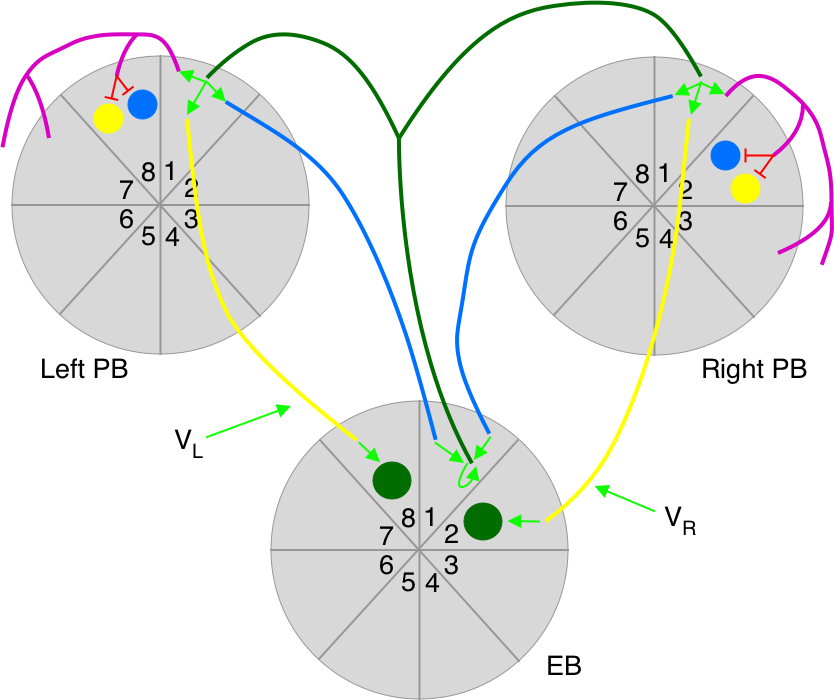
\includegraphics[width = 1.0\linewidth, trim={0 0 0 0}, clip=true]{../figures/model_structure.png}
		%\subcaption{Structure of the firing rate model. Green: EPG, blue:PEG, yellow:PEN1, purple:D7.}
		%\label{fig:struc}	
	\end{subfigure}
%	\hspace{0.1\linewidth}
%	\begin{subfigure}[t]{0.43\linewidth}
%		\centering
%		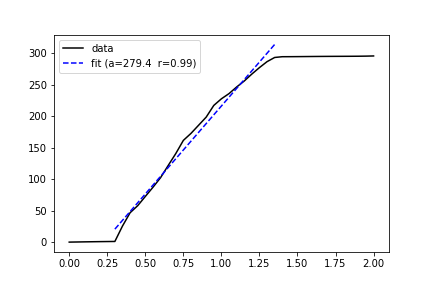
\includegraphics[width = 1.0\linewidth, trim={0 0 0 0}, clip=true]{../figures/testvels_late.png}
%		\caption{For small inputs, turning is not sustained. If we equilibrate for 2000ms and measure rotational velocity over 10000 ms, this threshold behavior is more evident.}
%		\label{fig:laterot}
%	\end{subfigure}
\caption{Structure of the firing rate model. Green: EPG, blue: PEG, yellow: PEN1, purple: D7.}
\label{fig:struc}
\end{figure}

I have used a tanh transfer function throughout and we constrain all firing rates to be $\geq 0$.
\begin{equation}
f(x) = tanh(x)
\end{equation}
Activities are then given by:
\begin{equation}
\tau_{EPG} \dfrac{dEPG}{dt} = -EPG + f(W_{PEG,EPG}\cdot PEG + W_{PEN1_L,EPG}\cdot PEN1_L + W_{PEN1_R,EPG}\cdot PEN1_R + W_{EPG,EPG}\cdot EPG)
\end{equation}
\begin{equation}
\tau_{PEG} \dfrac{dPEG}{dt} = -PEG + f(W_{EPG,PEG}\cdot EPG - W_{D7,PEG}\cdot D7 )
\end{equation}
\begin{equation}
\tau_{D7} \dfrac{dD7}{dt} =-D7 + f(W_{EPG,D7}\cdot EPG)
\end{equation}
\begin{equation}
\tau_{PEN1} \dfrac{dPEN1_L}{dt} = -PEN1_L + f(W_{EPG,PEN1_L}\cdot EPG - W_{D7,PEN1_L}\cdot D7 + v_L )
\end{equation}
\begin{equation}
\tau_{PEN1} \dfrac{dPEN1_R}{dt} = -PEN1_R + f(W_{EPG,PEN1_R}\cdot EPG - W_{D7,PEN1_R}\cdot D7 + v_R )
\end{equation}


\newpage


\section*{Velocity integration}

Velocity tuning curves are linear-ish and can be used to translate between real velocity in degrees/s and input velocity.
\begin{figure}[h]
	\centering
	\begin{subfigure}[t]{0.43\linewidth}
		\centering
		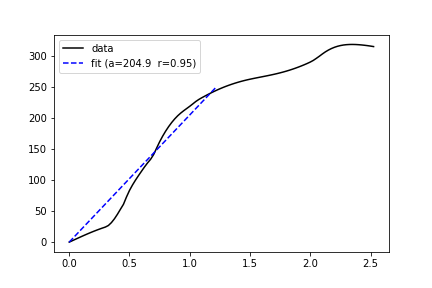
\includegraphics[width = 1.0\linewidth, trim={30 20 30 20}, clip=true]{../figures/testvels_early.png}
		\subcaption{equilibrate for 2000 ms, measure mean veocity over 500 ms $\rightarrow$ early velocity.}
		\label{fig:earlyrot}	
	\end{subfigure}
	\hspace{0.1\linewidth}
	\begin{subfigure}[t]{0.43\linewidth}
		\centering
		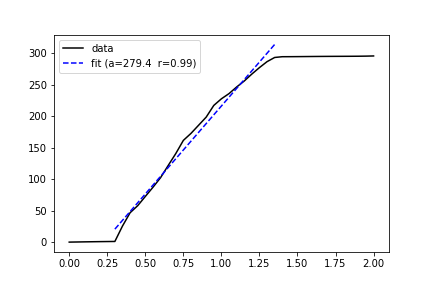
\includegraphics[width = 1.0\linewidth, trim={30 20 30 20}, clip=true]{../figures/testvels_late.png}
		\caption{For small inputs, turning is not sustained. If we equilibrate for 2000ms and measure rotational velocity over 10000 ms, this threshold behavior is more evident.}
		\label{fig:laterot}
	\end{subfigure}
\caption{ x-axis is input velocity ($v_R$), y axis is bump angular velocity (degrees/s)}
\label{fig:fit}
\end{figure}

Turns are generally short and slower than 200 degrees/s in the experimental data, and I therefore use a conversion of 200 based on figure \ref{fig:earlyrot} to go from experimental velocity to input velocity in equations 5 and 6.

\section*{Tracking experimental data}

We can simulate experimental data reasonably well even with this simple model.

\begin{figure}[h]
	\centering
	\begin{subfigure}[t]{0.46\linewidth}
		\centering
		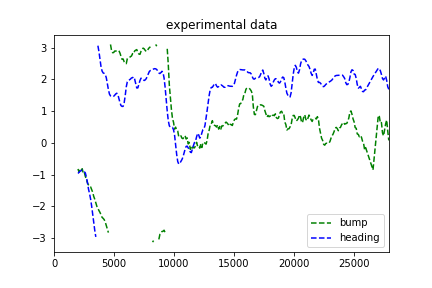
\includegraphics[width = 1.0\linewidth, trim={40 20 40 20}, clip=true]{../figures/real_heading.png}
		\subcaption{real heading and bump position}
		\label{fig:real_head}	
	\end{subfigure}
	\hspace{0.05\linewidth}
	\begin{subfigure}[t]{0.46\linewidth}
		\centering
		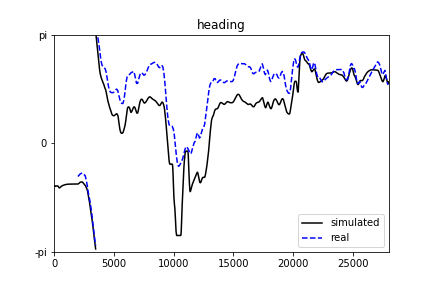
\includegraphics[width = 1.0\linewidth, trim={40 20 40 20}, clip=true]{../figures/sim_head.png}
		\caption{real heading and simulated bump position}
		\label{fig:head}
	\end{subfigure}
\caption{}
\label{fig:real_head_vel}
\end{figure}

\newpage
The heading curves in figure \ref{fig:head}  match reasonably well, as do the velocity curves in figure \ref{fig:vel}.

\begin{figure}[h]
	\centering
	\begin{subfigure}[t]{0.63\linewidth}
		\centering
		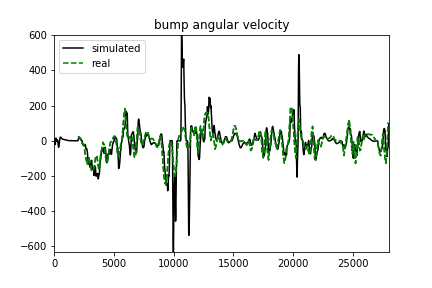
\includegraphics[width = 1.0\linewidth, trim={0 0 0 0}, clip=true]{../figures/sim_vel.png}
		\subcaption{real and simulated velocity curves}
		\label{fig:vel}	
	\end{subfigure}
%	\hspace{0.1\linewidth}
%	\begin{subfigure}[t]{0.63\linewidth}
%		\centering
%		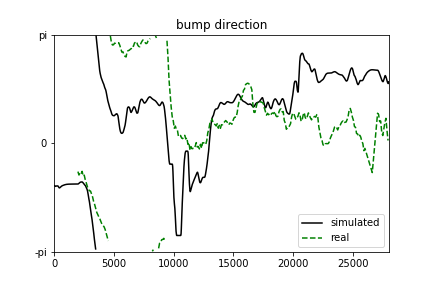
\includegraphics[width = 1.0\linewidth, trim={0 0 0 0}, clip=true]{../figures/sim_bump.png}
%		\caption{real bump and simulated bump}
%		\label{fig:bump}
%	\end{subfigure}
\caption{}
\label{fig:model}
\end{figure}

We see that our integrator does not quite follow the long rapid turns at 5,000ms and 10,000ms; but neither does the real bump (figure \ref{fig:real_head}) which actually does a worse job recovering from the turn.

The poor performance can result from very rapid turns leading to strong global PEN1 and thus EPG excitation, which in turn mediates D7 excitation and global inhibition. Thus broad excitation leads to downstream global inhibition and quenching of the bump (figure \ref{fig:quench}). This is different from the real system where the bump intensity tends to correlate positively with rotational velocity...\\
Local EPG - EPG recurrence in the EB somewhat mitigates this by retaining activity during strong inhibition of PEN1 and PEG.

%\newpage


\begin{figure}[h]
	\centering
	\begin{subfigure}[t]{0.47\linewidth}
		\centering
		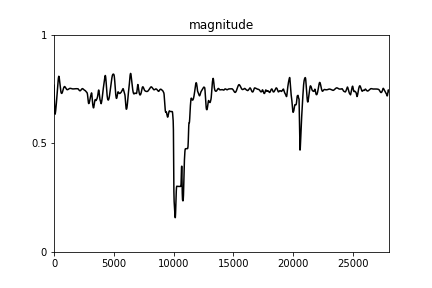
\includegraphics[width = 1.0\linewidth, trim={40 20 40 20}, clip=true]{../figures/sim_mag.png}
		\subcaption{Magnitude of PVA average. This decreases strongly following global inhibition near the rapid turn at 10,000 ms}
		\label{fig:mag}	
	\end{subfigure}
	\hspace{0.04\linewidth}
	\begin{subfigure}[t]{0.47\linewidth}
		\centering
		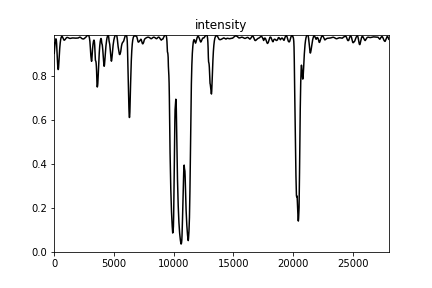
\includegraphics[width = 1.0\linewidth, trim={40 20 40 20}, clip=true]{../figures/sim_int.png}
		\caption{Intensity of the most active EPG neuron (bump height). This decreases strongly following global inhibition near the rapid turn at 10,000 ms.}
		\label{fig:int}
	\end{subfigure}
\caption{}
\label{fig:quench}
\end{figure}


\newpage

\section*{Shibire simulations}

On the basis of the above model we can simulate 'shibire inhibition' by inhibiting the outputs of a given neuron class. This is exemplified in figure \ref{fig:seqshi} where progressively stronger D7 inhibtion from 0\% to 70\% decreases the PVA magnitude of the EPG bump.

\begin{figure}[h]
	\centering
	\begin{subfigure}[t]{0.63\linewidth}
		\centering
		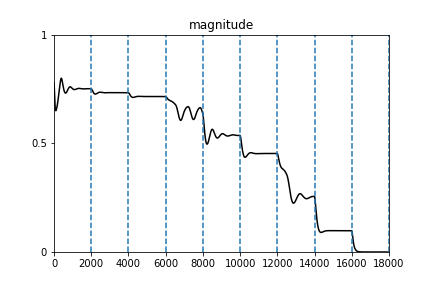
\includegraphics[width = 1.0\linewidth, trim={0 0 0 0}, clip=true]{../figures/D7_sequential_mags.png}
		%\subcaption{}
		%\label{fig:seqshia}	
	\end{subfigure}
	\hspace{0.1\linewidth}
%	\begin{subfigure}[t]{0.73\linewidth}
%		\centering
%		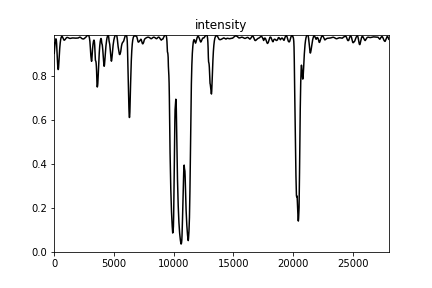
\includegraphics[width = 1.0\linewidth, trim={0 0 0 0}, clip=true]{../figures/sim_int.png}
%		\caption{intensity of the most active EPG neuron (bump height). This decreases strongly following global inhibition near the rapid turn at 1000 ms.}
%		\label{fig:dF}
%	\end{subfigure}
\caption{magnitude of PVA average  for sequential shibire inhition (0, 10\%, 20\%, ... , 70\%).}
\label{fig:seqshi}
\end{figure}

We can plot the distribution of EPG acitvity towards the end of each epoch to see how this changes (figure \ref{fig:D7dist}), and note that while the maximum bump intensity remains constant, decreased lateral inhibition leads to a broadening of the bump (what does the experimental data look like?).

\begin{figure}[h]
	\centering
	\begin{subfigure}[t]{0.32\linewidth}
		\centering
		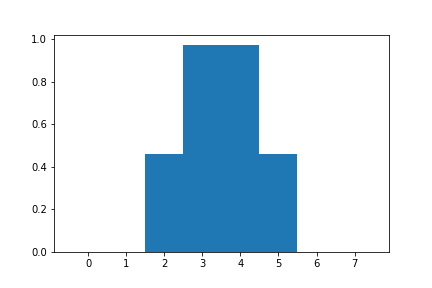
\includegraphics[width = 1.0\linewidth, trim={20 20 20 20}, clip=true]{../figures/D7_inhib_10.png}
		\subcaption{No inhibition}
		\label{fig:dist0}	
	\end{subfigure}
	\hspace{0.001\linewidth}
	\begin{subfigure}[t]{0.32\linewidth}
		\centering
		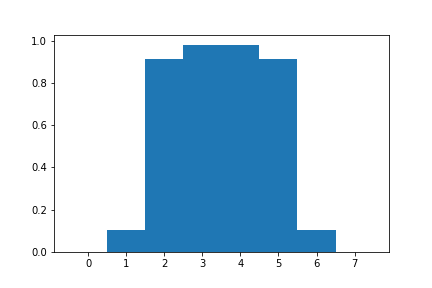
\includegraphics[width = 1.0\linewidth, trim={20 20 20 20}, clip=true]{../figures/D7_inhib_07.png}
		\caption{30\% D7 inhibition}
		\label{fig:dist30}
	\end{subfigure}
	\hspace{0.001\linewidth}
	\begin{subfigure}[t]{0.32\linewidth}
		\centering
		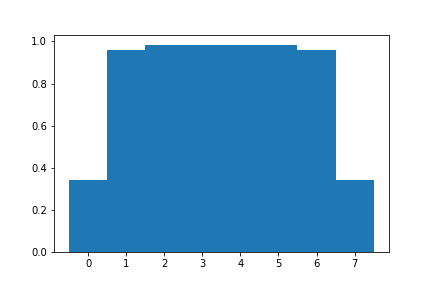
\includegraphics[width = 1.0\linewidth, trim={20 20 20 20}, clip=true]{../figures/D7_inhib_04.png}
		\caption{60\% D7 inhibition}
		\label{fig:dist60}
	\end{subfigure}
\caption{x axis is EB tile number, y axis is EPG activity}
\label{fig:D7dist}
\end{figure}

\newpage

This also decreases the ability of the bump to track the heading (figure \ref{fig:trackD7}), although not as much as we might expect from experimental data (i.e. the model is not very sensitive to changes in this direction of parameter space).

\begin{figure}[h]
	\centering
	\begin{subfigure}[t]{0.48\linewidth}
		\centering
		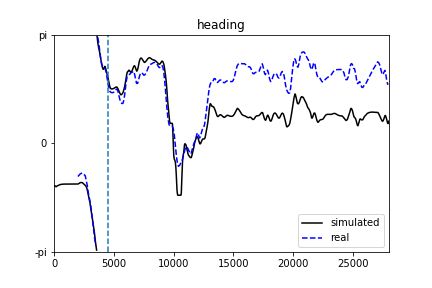
\includegraphics[width = 1.0\linewidth, trim={0 0 0 0}, clip=true]{../figures/sim_head_D7_07.png}
		\subcaption{30\% D7 inhibition}
		\label{fig:D730}	
	\end{subfigure}
	\hspace{0.01\linewidth}
	\begin{subfigure}[t]{0.48\linewidth}
		\centering
		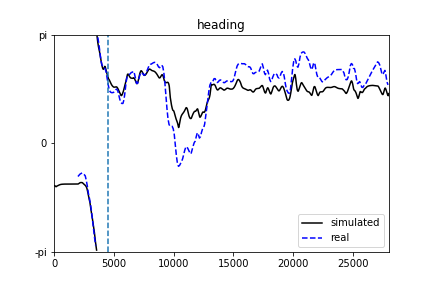
\includegraphics[width = 1.0\linewidth, trim={0 0 0 0}, clip=true]{../figures/sim_head_D7_04.png}
		\caption{60\% D7 inhibition}
		\label{fig:D760}
	\end{subfigure}
\caption{vertical line indicates time of inhibition (4500 ms).}
\label{fig:trackD7}
\end{figure}


The model is more sensive to inhibition of PEN1 outputs and also relatively robust to PEG inhibition (figure \ref{fig:trackPP})

\begin{figure}[h]
	\centering
	\begin{subfigure}[t]{0.48\linewidth}
		\centering
		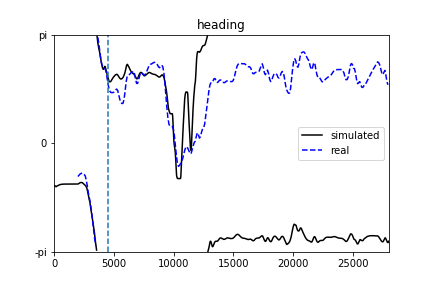
\includegraphics[width = 1.0\linewidth, trim={0 0 0 0}, clip=true]{../figures/sim_head_PEN1_07.png}
		\subcaption{30\% PEN1 inhibition}
		\label{fig:F}	
	\end{subfigure}
	\hspace{0.01\linewidth}
	\begin{subfigure}[t]{0.48\linewidth}
		\centering
		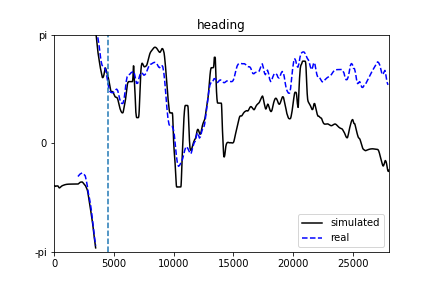
\includegraphics[width = 1.0\linewidth, trim={0 0 0 0}, clip=true]{../figures/sim_head_PEG_07.png}
		\caption{30\% PEG inhibition}
		\label{fig:dF}
	\end{subfigure}
\caption{vertical line indicates time of inhibition (4500 ms).}
\label{fig:trackPP}
\end{figure}

\newpage

\section*{Code}

fr\_class.py\\
implements the 'frmodel' class that is used for all simulations, storing weights and activities etc. Also has methods for calculating PVAs and plotting some different aspects of a simulation. The 'add\_event' method allows for planning of changes in rotational velocity or shibire inhibition at particular timepoints.

analysis\_functions.py\\
Simple functions for constructing velocity curves and carrying out sequential shibire inhibitions.

run\_example\_simulation.py\\
Contains a function for loading experimental data for a single fly and comparing this to simulated data.



%\lstinputlisting[language=python]{../fr_class.py}

\end{document}